\documentclass{article}





\usepackage[english]{babel}
\usepackage{blindtext}



\title{A caption test}
\author{Some one}
\date{\today}



\usepackage{caption}
\usepackage[dvipdfmx]{graphicx}
\usepackage{subcaption}
\usepackage{float}


\begin{document}


\setlength\fboxsep{0pt}
\setlength\fboxrule{0.5pt}

\begin{figure}
\begin{tabular}{cc}
  \begin{subfigure}[b]{0.5\textwidth}   % l   b   r   t
  \fbox{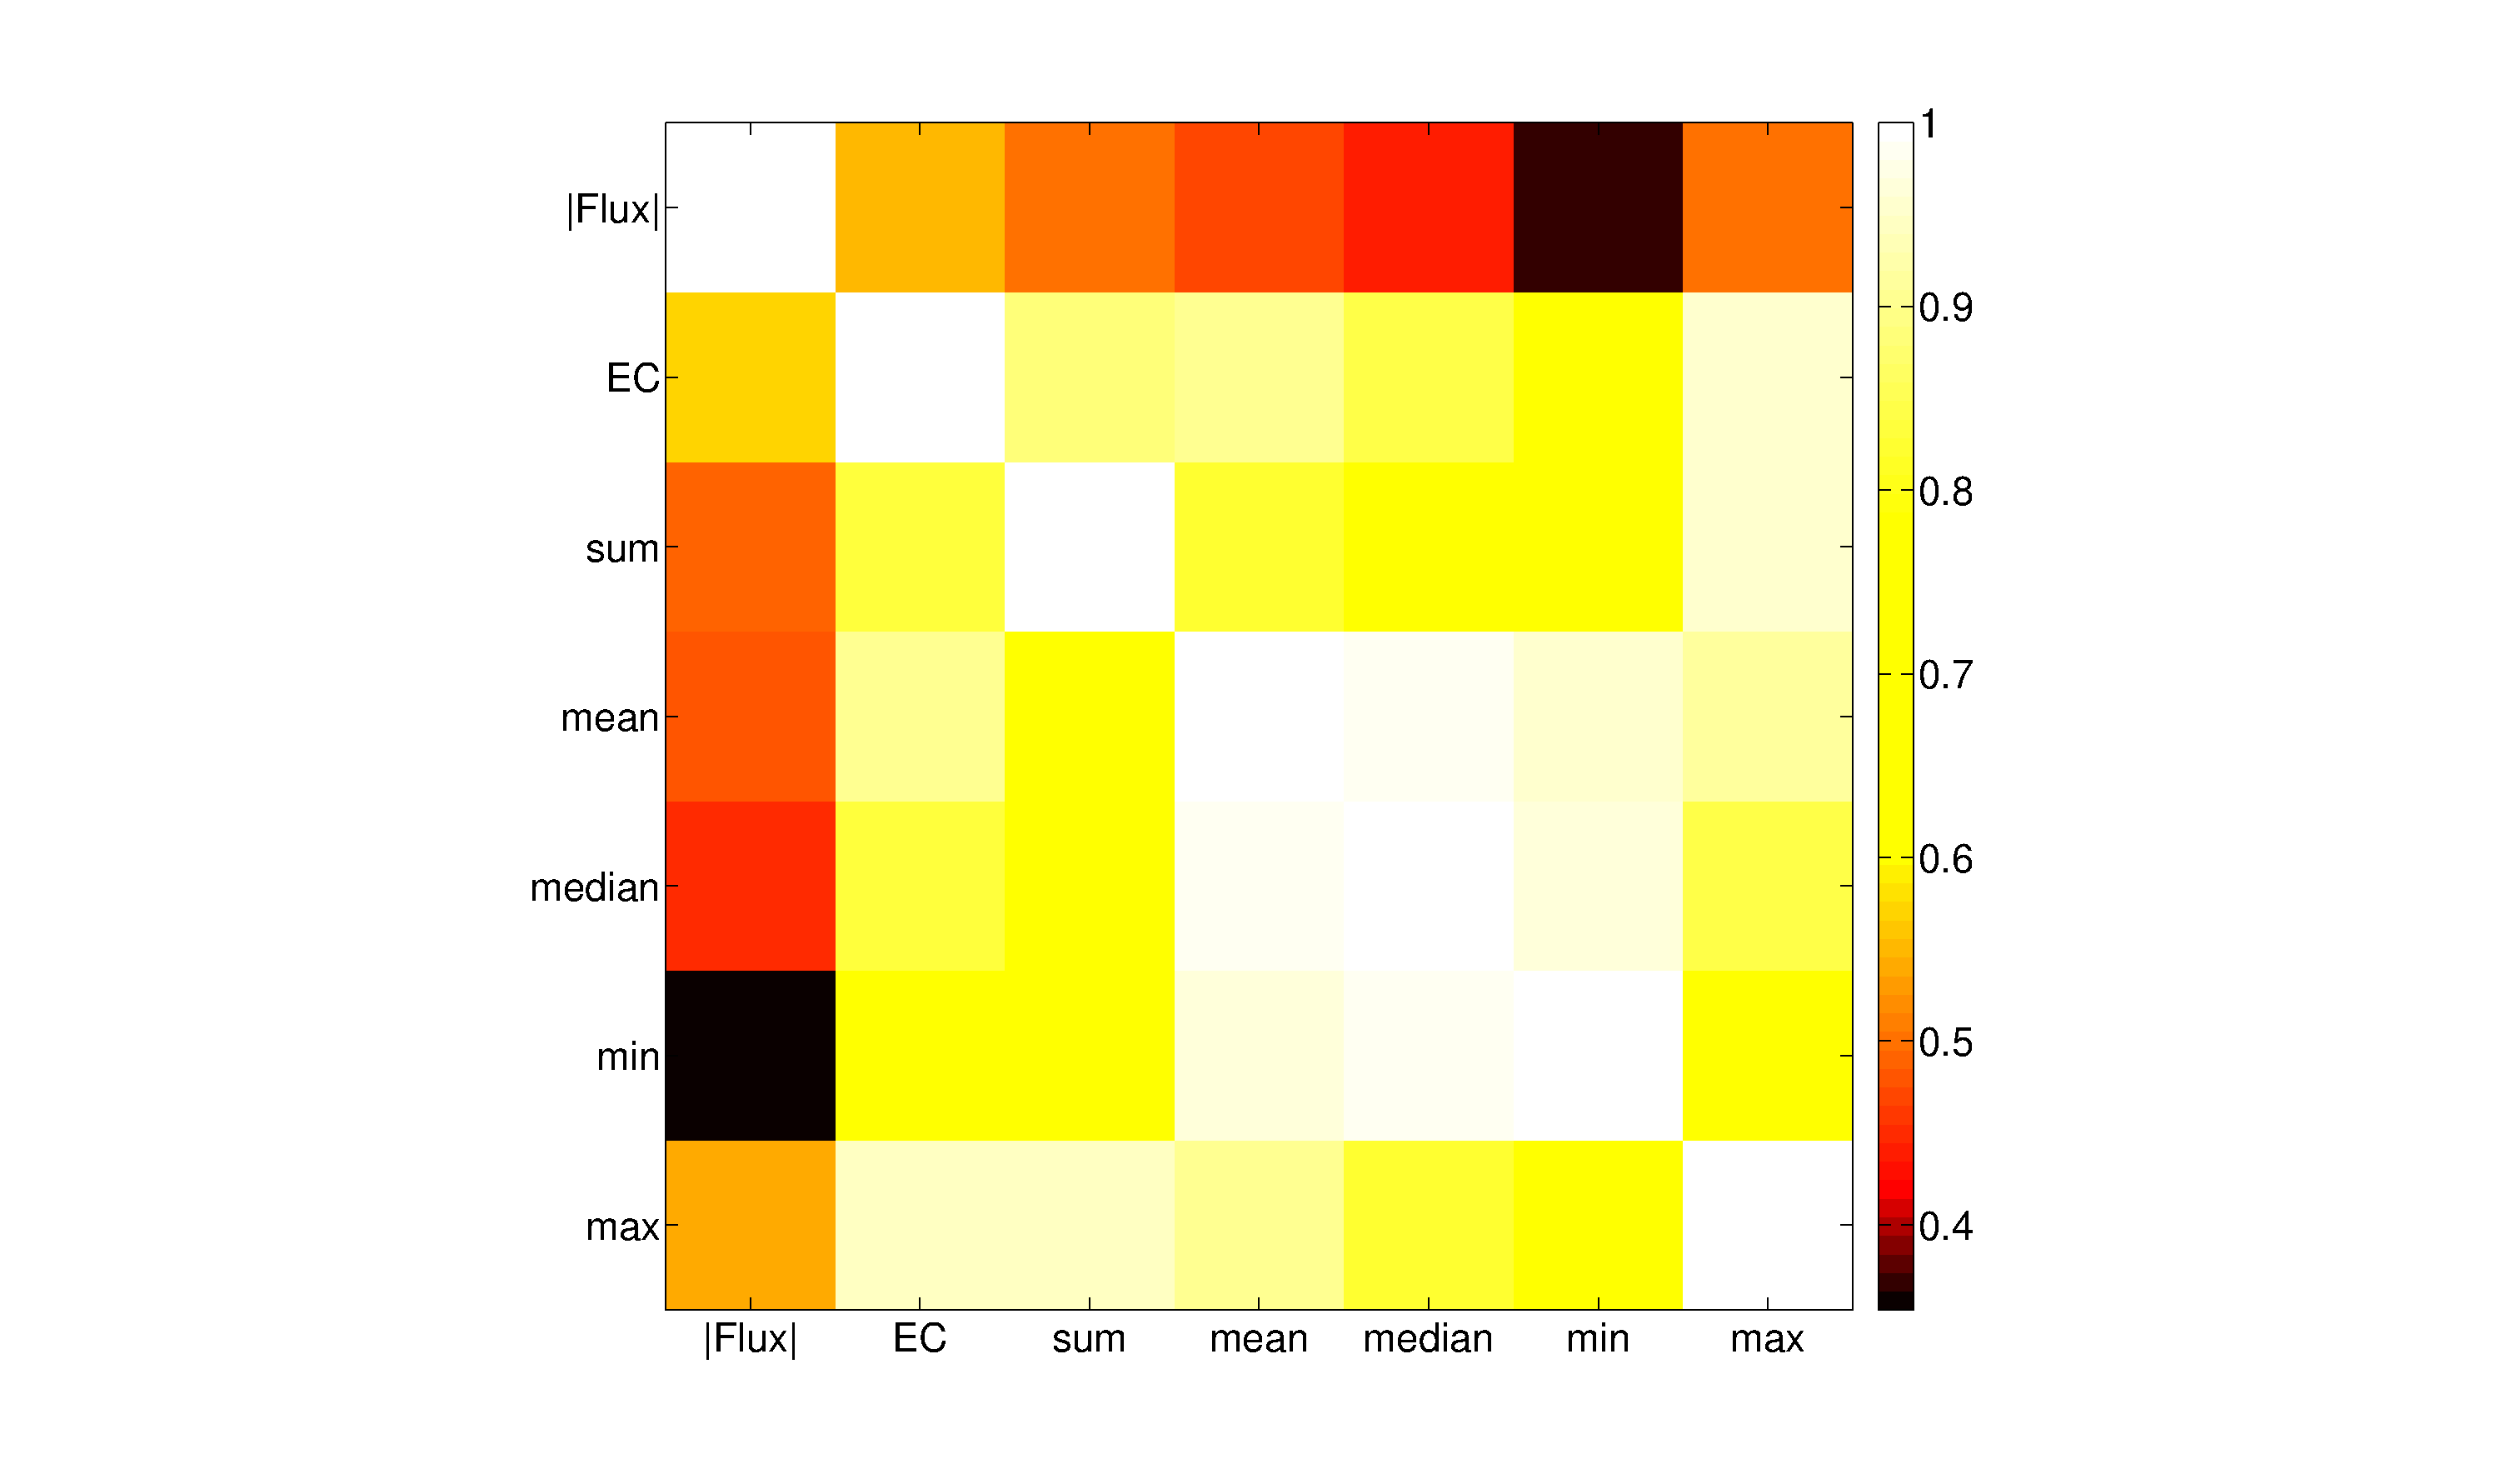
\includegraphics[width=\textwidth, trim=25cm 3cm -5cm 0cm, clip=true]
    {YeastExpFluxCompare}}
  \vspace{3mm} \caption{Yeast} \label{fig:FluxExpCmp:A}
  \end{subfigure}
&
  \begin{subfigure}[b]{0.5\textwidth}
  \fbox{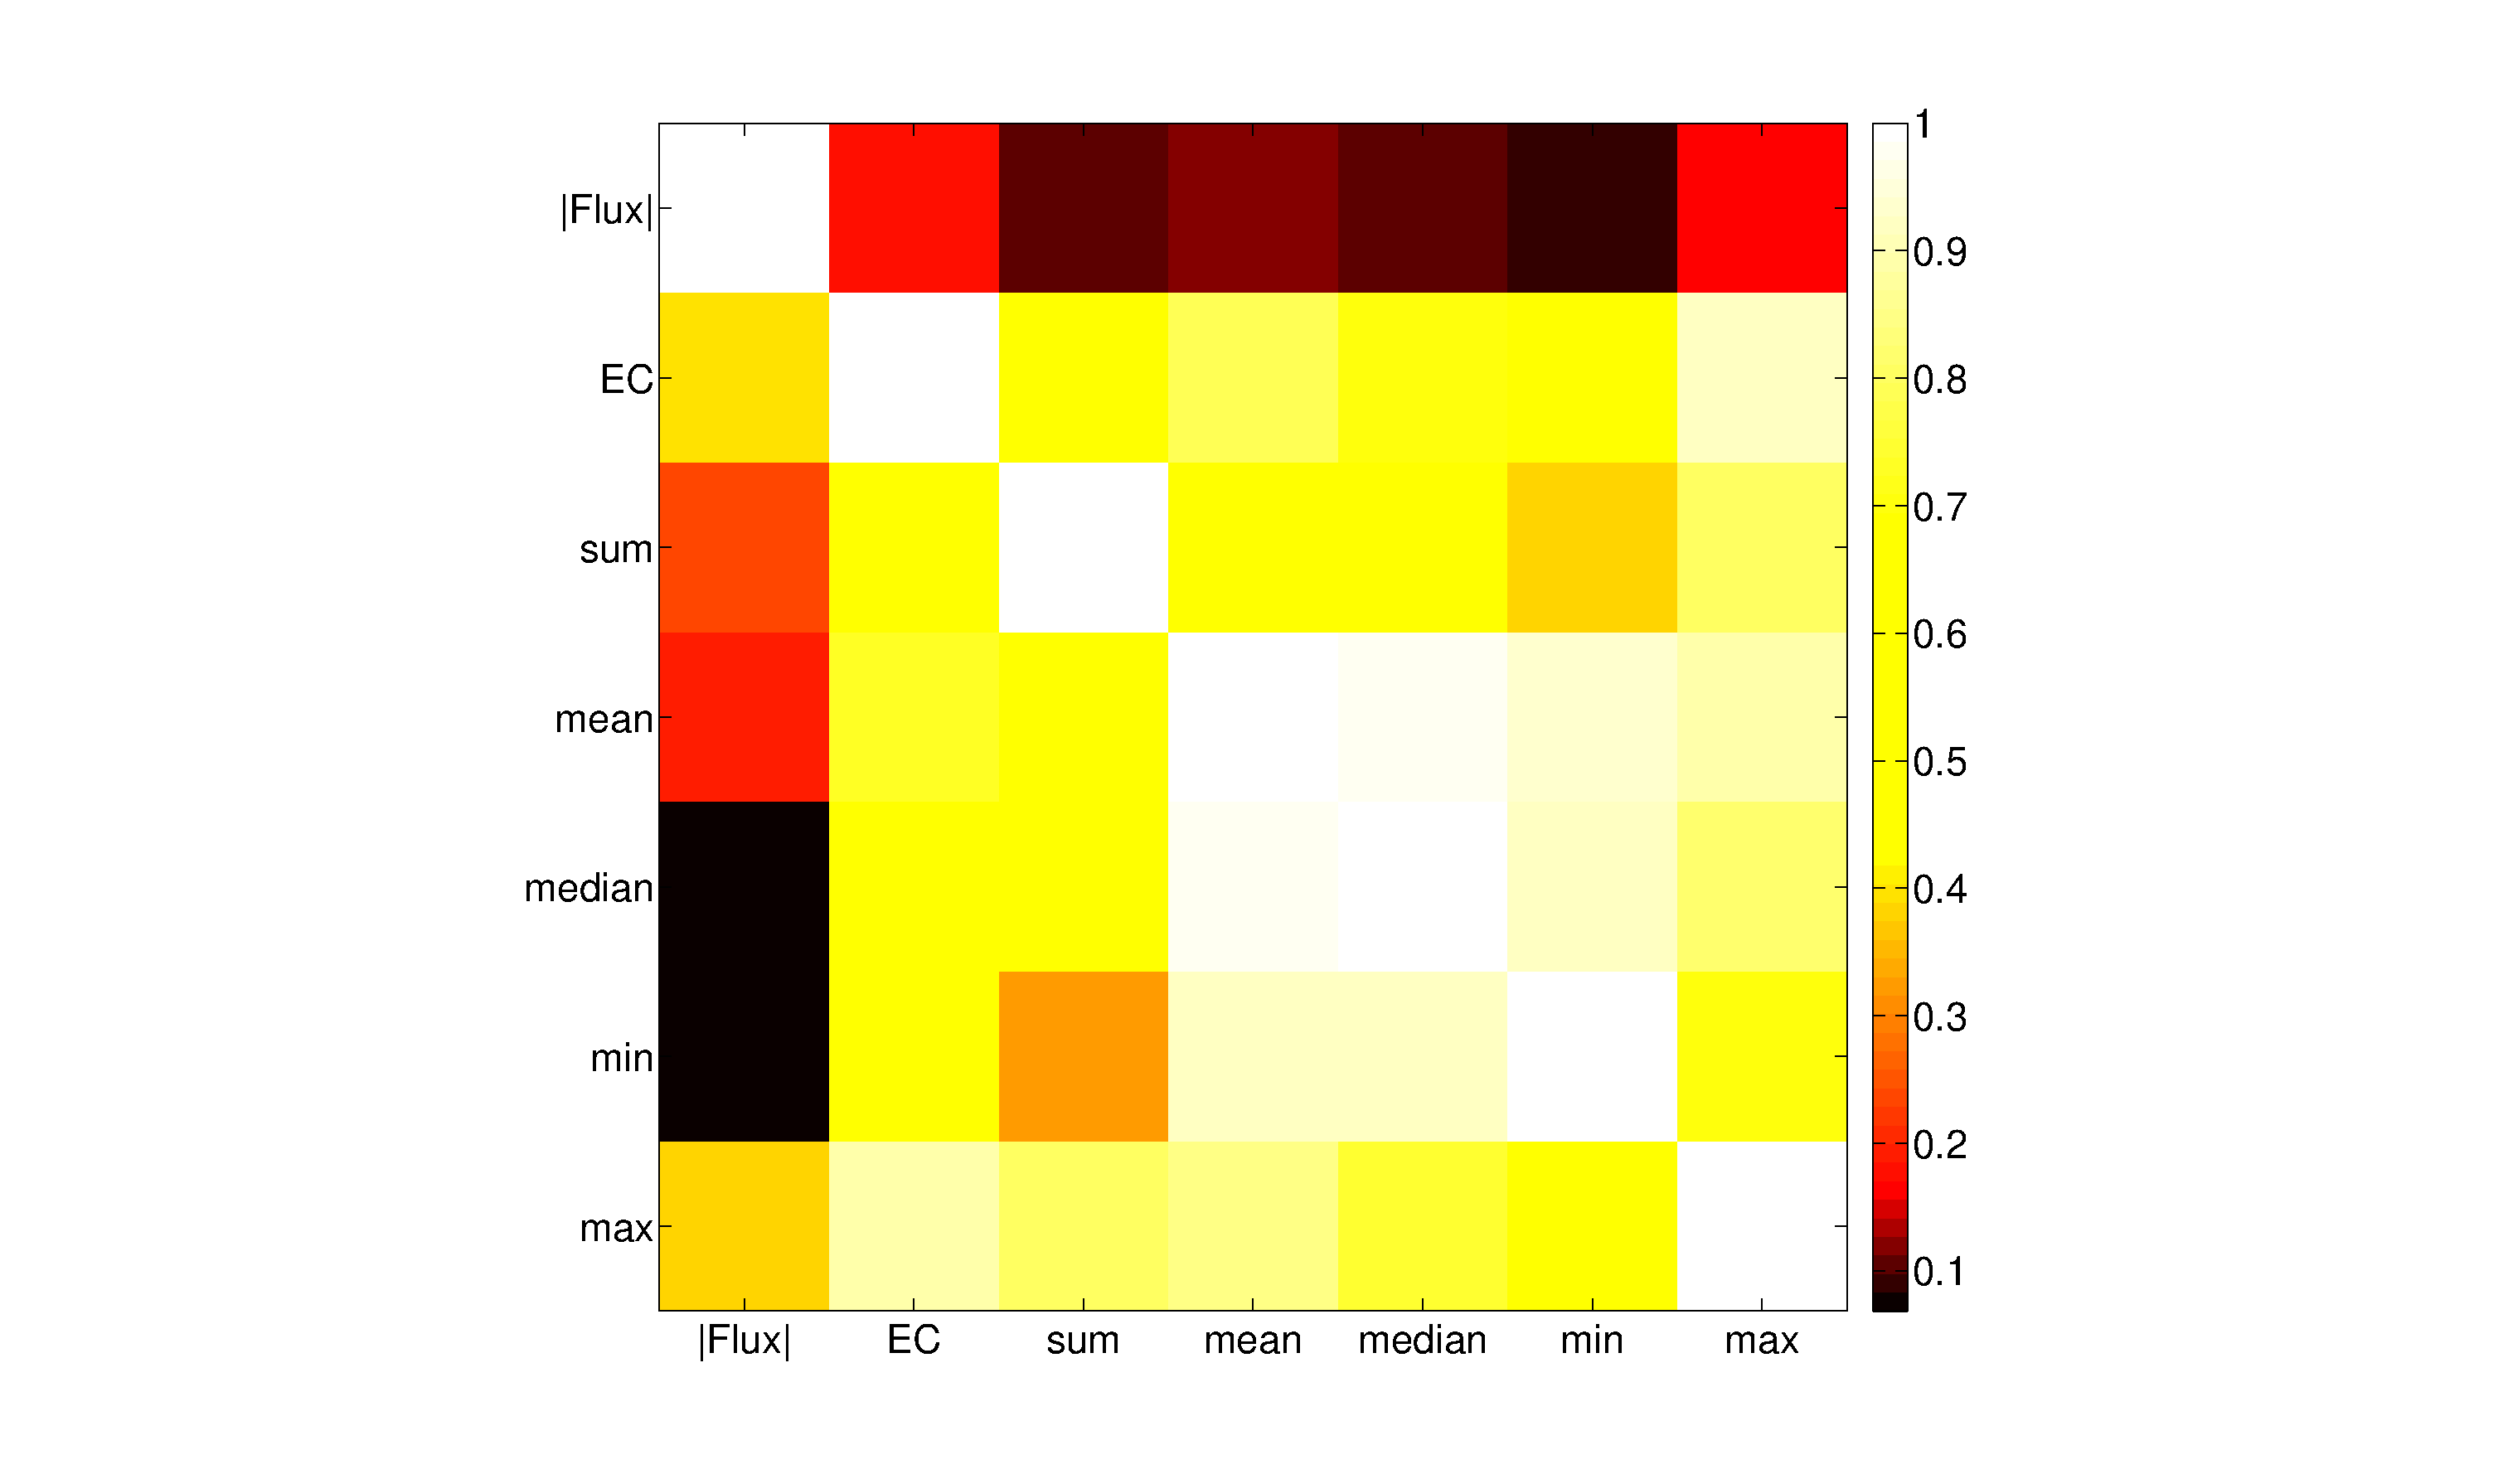
\includegraphics[width=\textwidth, trim=25cm 3cm -5cm 0cm, clip=true]
    {HumanExpFluxCompare}}
  \vspace{3mm} \caption{Human} \label{fig:FluxExpCmp:B}
  \end{subfigure}
\\
\end{tabular}
\caption{\blindtext}
\label{fig:FluxExpCmp}
\end{figure}

Please refer to Supporting Table~\ref{fig:FluxExpCmp}.

\end{document}
